\resetgraphicspath
\appendtographicspath{{./Introduction/figures}}
\appendtographicspath{{./Chapter 1/figures/} }
\appendtographicspath{{./Chapter 1/islands} }
\appendtographicspath{ {./Chapter 3/figures/erosion/}{./Chapter 3/figures/terrain_representations/}{./Chapter 3/results/}{./Chapter 3/otherPapersRepro/} {./Chapter 3/images/erosion-processes/}}

\chapter{Background}
\label{chap:background}
\minitoc

The purpose of this chapter is to establish the common ground required for understanding the remainder of this thesis. Because the three contributions presented in this thesis each come with their own specialised state of the art, the role of this chapter is not to provide an exhaustive survey of algorithms, but rather to:
\begin{Itemize}
    \Item{} introduce the key concepts and terminology shared across all contributions;
    \Item{} clarify the main terrain representations and interaction paradigms relevant to procedural modelling;
    \Item{} highlight the biological and ecological principles of coral reefs that directly constrain modelling choices;
    \Item{} outline the challenges specific to underwater landscape synthesis that motivate the research directions pursued in this work.
\end{Itemize}





Procedural generation of environments sits at the intersection of realism, speed, and user control. Achieving all three simultaneously remains an open challenge, particularly in the context of coral reef islands where terrain is co-constructed by geological processes, hydrodynamics, and living organisms. Understanding how existing approaches position themselves along this speed-realism-control triangle will provide a framework for situating our own contributions.

A second cross-cutting issue is the choice of representation. From heightmaps to voxels and layered models, each structure affords specific strengths (efficiency, volumetric detail, analytic flexibility) but also imposes limitations (no overhangs, high memory cost, restricted editing). Because each contribution in this thesis relies on a different representation, a concise overview is needed upfront to avoid duplication later.

Finally, modelling coral reef seascapes demands knowledge beyond computer graphics. The morphology and ecology of corals impose environmental constraints (light dependence, depth ranges, growth morphologies, competition with algae) that must be abstracted into procedural rules. In turn, the underwater setting introduces observational and modelling challenges, ranging from scarce volumetric data to fluid-biology feedbacks, that explain why existing terrestrial terrain methods cannot be directly transplanted.

Together, these elements form the conceptual scaffolding for the rest of the document. The chapter first reviews the foundations of procedural terrain generation, then examines terrain representations and interaction paradigms, before introducing coral biology and the distinctive challenges of underwater landscape modelling.

% This thesis dives in the domain of procedural underwater environment generation, falling at the intersection of procedural generation, terrain representation, terrain authoring and interactions, and underwater biology. In this chapter we introduce the basis for understanding the different notions used in the rest of the document. We first present the notion of procedural terrain generation which creates virtual landscapes to be used in the entertainment applications and scientific simulations with as few as possible user efforts, which will be the basis of our work all along. As the terrain data structure, or "terrain representation", has a critical importance over the algorithms of generation, interaction and simulation, we will overview the available representations used in the different chapters of this work, presenting the advantages and inconvenients of each structure. 

% User interactions means on generation spans from manually manipulating each triangle of a 3D model (giving too much work to the user) to fully automatic generation of the model (giving too few control on the result). A compromise must be found to strike a balance between realism and control. We propose an overview of the speed-realism-controllability challenge.

% Finally, this work being tailored for underwater environments surrounding coral reef islands, we provide an overview of coral biology and coral reef definitions.

\section{Procedural terrain generation}
\label{sec:state-of-the-art_procedural-generation}

Procedural generation consist of algorithmically creating content based on predefined rules, mathematical models, or data-driven methods, rather than authoring it manually. The key advantage include reducing storage needs (since content is generated on-the-fly), enabling rapid creation of large or varied content, and supporting both reproducibility and controlled variability. These benefits are especially valuable in terrain generation where large landscapes or seascape can be created from compact parameters sets where artists or researchers can iterate quickly towards a desired output through as few trials and errors as possible.

\AltTextImage{
The conceptual roots of procedural techniques in graphics trace back to fractal geometry (see \cref{fig:intro-fractal}) and noise functions (see \cref{fig:intro-noises}). Mandelbrot's work on fractals demonstrated how complex, self-similar structures can arise from simple rules and randomness, influencing landscape modelling approaches that mimic natural roughness and multi-scale detail \cite{Mandelbrot1983}. Perlin's introduction of gradient noise provided a practical mechanism to generate coherent pseudo-random patterns for textures and terrain features \cite{Perlin1985}. These foundational ideas underpin many terrain algorithms, where noise at multiple scales produces hills, valleys, and finer details.
}{Snowflake5-Siertriangle11.jpg}{Fractal geometry: Sierpinski Triangle in Koch Snowflake, from Larry Riddle}{fig:intro-fractal}

\AltTextImage{
    Procedural paradigms are often categorised as deterministic (repeatable given fixed inputs), stochastic (introducing randomness for variation), or hybrid (structure defined by deterministic rules, with randomness filling details). Rule-based systems, where content emerges via iterative application of predefined rules or grammars, play a central role in procedural generation, particularly in generating structured features (e.g., river networks, vegetation patterns). In terrain generation, deterministic components ensure global coherence (e.g., major landmass shapes), while stochastic elements add natural variability (e.g., subtle elevation perturbations). Methods proposed in later chapters leverage these paradigms: for instance, the sketch-based island method, combined with noise and data-driven augmentation from \cref{chap:coral-island} yields varied yet controlled outputs, and our ecosystem generator presented \cref{chap:semantic-representation} is governed by rule-based systems with stochastic sampling.
}{noises.pdf}{Example of procedural noises}{fig:intro-noises}
    
Recent advances have started integrating machine learning to learn distributions of terrain patches or entire landscapes from data, enabling synthesis of realistic terrain patterns beyond hand-tuned noise parameters, using especially generative models such as GANs or autoencoders. In \cref{chap:coral-island} we use a conditional GAN to diversify coral island heightmaps. However, a detailed description of learning-based terrain methods appears in that chapter's State-of-the-Art.

In interactive and production pipelines, procedural systems must balance realism, speed, and user control. Fast evaluation (often parallelised and/or using GPU) supports real-time or near-interactive feedback for artist-driven editing. Parameter design and UI tools (e.g., sketching, semantic objects, masking) are critical to let users influence generation intuitively. The semantic \glosses{EnvObj} framework proposed in \cref{chap:semantic-representation} exemplifies user-centric design, enabling multi-scale editing and expert knowledge integration.

Procedural terrain generation also encompasses physical simulation techniques such as erosion and sediment transport models, that refine initial shapes to enhance plausibility. These simulations are typically more expensive but can run offline or via parallel algorithms. \cref{chap:erosion} presents a particle-based erosion method applicable across representations (height fields, voxels, etc.), reflecting this integration of procedural and physical approaches.


Terrain refers to the physical features and configuration of a specific area of land. It includes the elevation, slope, and the overall topography (e.g., mountains, valleys, plains, ...). Terrain is often used to describe the surface characteristics of the land, focusing on the natural contours and the geographical aspects that define a region's physical form.

\AltTextImage{
    While the term "terrain" describes the physical characteristics of land, it does not include the natural elements that shape an area's identity. Elements such as vegetation, water bodies, and climatic conditions are essential our perception and understanding of landscapes. Therefore, when discussing procedural generation in virtual environments, "landscape generation" is a more fitting term, as it integrates these natural elements along with the topographical features.

    In addition to "terrain generation", other terms such as "landscape generation", "world generation", and "environment generation" can be used to describe the creation of virtual landscapes. These terms are interchangeable and all refer to the process of generating physical terrain along with natural and artificial elements. However, by convention and for simplicity, the term "terrain generation" is most commonly used in the Computer Graphics field. Despite its original focus on the physical features of the land, "terrain generation" has evolved to encompass a broader range of environmental elements, making it a convenient and widely accepted term for describing the comprehensive process of creating virtual environments.

}{Multi-representations-at-once-heightmap.png, Multi-representations-at-once-divided.png}{An initial height map (top) can be converted into multiple terrain representations (bottom, from left to right): discrete height field, layered model, density-voxel model (rendered with Marching Cubes), binary-voxel model}{fig:intro-multiple-representations}

The terrain shown in \cref{fig:intro-multiple-representations} has been converted into different representations we used in our works; next section presents these representations with their main advantages and inconvenients.



\section{Terrain representations}
A terrain can be represented in many different ways (see \cref{fig:intro-multiple-representations}, which shows four examples), each suited to particular algorithms and interaction paradigms. Because converting from one representation to another generally incurs information loss, choosing an appropriate underlying model is crucial for the quality and controllability of procedural results. This chapter therefore introduces only the models that will be used in the remainder of the thesis; the reader is referred to \cite{Galin2019} for a comprehensive survey.

% \paragraph*{Other representations.}
For completeness, we note that several families do not appear in our later chapters, including irregular meshes and TINs (Triangulated Irregular Networks), and point-based splats or surfels, or neural representations \cite{Yang2005, Zhu2008, Arnone2021, Atas2022, Chen2024, Chen2025, Dai2024, Li2022}. These alternatives are relevant in the broader terrain-modelling literature, but lie outside the scope of the procedural techniques developed in this thesis.

%---------------------------------------------------------------------
\subsection{2.5D representations (Elevation models)}
%---------------------------------------------------------------------

\begin{figure}
  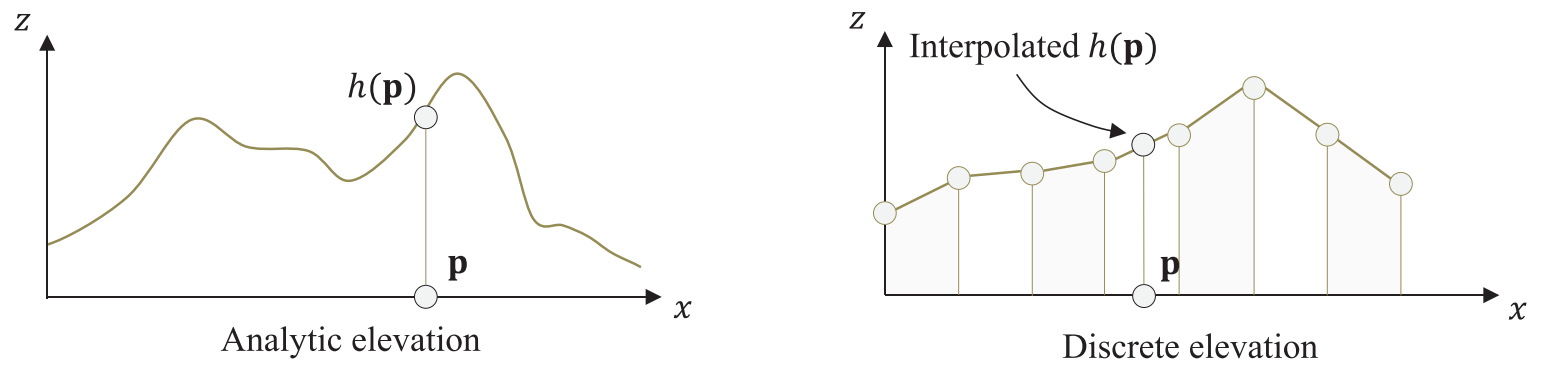
\includegraphics[width=.8\linewidth]{elevation_representation.png}
  \caption{Elevation models can be (left) implicit functions evaluated at any point, or (right) discrete samples augmented with interpolation to recover a continuous surface \cite{Galin2019}}
  \label{fig:erosion-elevation-representation}
\end{figure}

Elevation models describe the terrain by a height field $h : \R^{2}  \to  \R$, assigning a single elevation value to every planimetric location. Because each $(x,y)$ has only one height, such models cannot express overhangs or caves; we therefore refer to them as "2.5D". Mathematically, height fields are analogous to images, making them amenable to decades of image-processing techniques. Their favourable memory footprint and analytic simplicity explain their preponderance in open-world games, GIS, and remote sensing.

\begin{figure}
    \autofitgraphics[width=.5\linewidth]{Terrain_representations/heightmap_high-res_628x628.png}
    \autofitgraphics{Terrain_representations/heightmap_all-at-once.png}
    \caption{Top: an implicit height field can be ray-traced at any resolution. Bottom: discrete height fields (samples of the top
    function) have fixed resolution: finer meshes approach the implicit surface, whereas down-sampling inevitably loses detail.}
    \label{fig:sota-representations-heights-resolutions}
\end{figure}


%.....................................................................
\subsubsection{Discrete height fields}
%.....................................................................
Discrete height fields, often called "heightmaps", store sampled elevations on a regular grid (\cref{fig:intro-multiple-representations}, top). Formally, they are a function $h_{ \text{d}} : \mathbb{Z}^{2} \to \R$ defined only on integer lattice points. To render or analyse the terrain at arbitrary positions we reconstruct a continuous surface $ \tilde{h}_{ \text{d}} : \R^{2} \to \R$ using interpolation (linear, bilinear, bicubic, ...) (\cref{fig:erosion-elevation-representation}, right). Their raster nature aligns with GPUs and with convolutional neural architectures; our first contribution (\cref{chap:coral-island}) relies on this representation to fit the greyscale image format. Discrete grids scale to large terrains with modest memory footprint, but fixes the dimensions and resolution of the domain.

%.....................................................................
\subsubsection{Implicit height fields}
%.....................................................................
\AltTextImage{
    An implicit height field represents the terrain by a closed-form or procedural function $h_{ \text{i}} : \R^{2} \to \R$ that can be evaluated at any $(x,y)$ (\cref{fig:erosion-elevation-representation}, left). Because no samples are stored, the representation is compact and inherently multi-scale (in opposition of discrete height fields, as visible in \cref{fig:sota-representations-heights-resolutions}), and it supports analytic operations. % (derivatives, spectral synthesis, Booleans). 
    These properties make it the backbone of the semantic terrain synthesis developed in \cref{chap:semantic-representation}. The drawback is runtime cost: densely evaluating a complex function over a large domain is computationally expensive, but allow "on-demand" evaluation.
}{primitives_representation.png}{Primitives composition \cite{Genevaux2015}}{fig:erosion-primitives-representation}

Beyond the construction-tree model of \cite{Genevaux2015} (\cref{fig:erosion-primitives-representation}), several other implicit 2.5D terrain representations are commonly employed: gradient-noise fractals (e.g., Perlin, Simplex or FBM) provide fast, tileable, and stochastic detail; spectral or analytic formulas (e.g., ridge-noise, domain warps or erosion kernels) enable semantically tuned landforms ; feature-curve diffusion techniques allow users to define ridges and rivers via polylines which are then diffused into the height field ; vector-primitive models blend geometric shapes like ellipsoids or plates directly into the terrain surface ; and radial-basis-function (RBF) implicits fit a sparse set of control points with smooth Hermite interpolants for interactive editing .

These alternatives are surveyed in depth in \cref{chap:coral-island}' State-of-the-Art.

%---------------------------------------------------------------------
\subsection{3D representations (Volumetric models)}
%---------------------------------------------------------------------
Volumetric models encode not only the terrain surface but also its interior, making it possible to represent overhangs, caves, voids, and material heterogeneity that 2.5D elevation models cannot capture.
We organise them into three families: implicit fields, discrete voxel grids, and layered models.

%.....................................................................
\subsubsection{Implicit volumetric models}
%.....................................................................
\AltTextImageR{
    An implicit model defines a signed or unsigned scalar field $f_{ \text{i}} : \R^{3} \to \R$; the terrain surface is the isosurface $f_{ \text{i}}(\mathbf x)=0$. Positive values typically denote solid matter, negative values air. Because the field is continuous, implicit models enable smooth blends, Constructive Solid Geometry (CSG) operations (\cref{fig:intro-CSG}), and multi-scale detail synthesis \cite{Paris2019a}. Their main drawbacks are the cost of dense evaluation and the need to polygonise (e.g.\ Marching Cubes) for rasterisation \cite{Araujo2015}.
}{Csg_tree.png}{CSG tree combining implicit primitives with intersection (left), unions (right) and difference (top) operations.}{fig:intro-CSG}
    
Signed-distance fields (SDFs) store the shortest distance to the surface and are widely used for real-time deformation and global illumination. Adaptively-sampled distance fields (ADF) \cite{Frisken2000} refine the grid where detail is needed, while sparse voxel SDFs such as OpenVDB scale to billions of voxels. Radial-basis implicit volumes offer smooth interpolation from scattered samples.

%.....................................................................
\subsubsection{Discrete voxel grid models}
%.....................................................................
A voxel grid partitions space into a regular lattice $\Z^{3}$; each lattice point $v=(i,j,k)$ stores a datum describing the local state of the terrain. Because grids are topologically simple and cache-friendly, they interface well with GPU rasterisers, cellular-automata solvers, and image-processing operators extended to 3-D. The main drawback is cubic memory growth; sparse and hierarchical encodings (SVO, DAG, OpenVDB) alleviate this when the occupied volume is far below the bounding box
\cite{Laine2010,Villanueva2017,Museth2013}.

Voxel grids support boolean set operations, distance transforms, morphological filters, and mesh extraction (Marching Cubes, Dual Contouring) in a very similar fashion as the their 2D conterparts in image processing (binary images, indexed images, and greyscale images).

\AltTextImage{
    %=====================================================================
    \subsubsubsection{Binary voxel grids}
    %=====================================================================
    Binary voxel grids record pure occupancy, defined as $o : \mathbb Z^{3} \to \{0,1\}$. Their single-bit payload makes them the lightest form of volumetric storage, and simple bit-packing enables SIMD flood-fills or cellular automata. When combined with Sparse Voxel Octrees or voxel DAGs they scale to scenes containing $10^{12}$ voxels while keeping GPU residency practical \cite{Laine2010,Villanueva2017}. The downside is blocky surfaces: without post-processing, silhouettes follow axis-aligned voxel faces (see \cref{fig:intro-voxels-binary-density}, left). Smoothing kernels or surface nets can mitigate this at the cost of losing exact occupancy.
}{voxels-binary-density.png}{Binary surface (left) vs.\ density-grid isosurface (right). Density grids preserve curved boundaries without refining the lattice.}{fig:intro-voxels-binary-density}


\AltTextImage{
    %=====================================================================
    \subsubsubsection{Material voxel grids}
    %=====================================================================
    Material grids extend binary occupancy with categorical information (stone, sand, water, ...) with $\mu : \mathbb Z^{3} \to \mathcal M$ (with $\mathcal M$ a material from a finite material set). They are the volumetric analogue of indexed images and form the basis of block-based worlds such as \citeProgram{Minecraft2011} (\cref{fig:intro-material-voxels-minecraft}). Each update affects exactly one cell, making editing and cellular-automata simulation intuitive. The obvious limitation is abrupt boundaries: transitions remain voxel-aligned.
}{material-voxels-minecraft.png}{Each cell of the voxel grid is encoded with a material, visible by different textures. }{fig:intro-material-voxels-minecraft}

%=====================================================================
\subsubsubsection{Density voxel grids}
%=====================================================================
Storing a real-valued scalar per voxel enables implicit isosurfaces inside the grid, defined as $d : \mathbb Z^{3} \to \R$ with $d$ typically an occupacy fraction or a signed distance. Marching Cubes or Dual Contouring produce triangle meshes with sub-voxel geometric accuracy (\cref{fig:intro-voxels-binary-density}, right), while the grid still supports topology-aware editing via direct field arithmetic. Applications range from high-fidelity VFX terrain in OpenVDB \cite{Museth2013} to destructive game mechanics and GPU-based fluid coupling. Memory cost is higher (4 or 8 bytes per voxel), but sparsity structures or narrow-band storage tame the overhead \cite{Frisken2000}.



%.....................................................................
\subsubsection{Layered models}
%.....................................................................
\AltTextImage{
    \cite{Benes2001} introduced a layered-based terrain representation in which the landscape is discretized as a 2D grid of vertical material stacks, each composed of horizontal strata representing a single homogeneous material (e.g., water, sand, bedrock, ... presented in \cref{fig:intro-layers}). The terrain surface is given by the height of the top layer in each stack. 
}{Layer-representation.png}{Layer representation as described in \cite{Benes2001}. \cite{Peytavie2009b} allows air and water strata to be inserted between solid material strata. }{fig:intro-layers}
\AltTextImage{
    \cite{Peytavie2009b} improved the structure in two critical ways. First, they introduce an explicit air layer that may be inserted between solid strata to allow true 3D features such as caves, overhangs, and arches. Second, they couple this discrete stack data with a convolution-based implicit surface field $f(\p)$, defined as the normalized local volume fraction of solid material $\mathcal{V}_\mathcal{M}$ within a cubic kernel $\mathcal{V}_\Omega$. The zero-level set $\mathcal{V}_\mathcal{M} = \frac{1}{2} \mathcal{V}_\Omega$ is polygonized to form a smooth, editable surface mesh (see \cref{fig:intro-layers-hybrid}, using the empty volume $\mathcal{V}_\emptyset = \mathcal{V}_\Omega - \mathcal{V}_\mathcal{M}$). 
}{Terrain_representations/Layer-representation-implicit.png}{The implicit volume (right, red) computed from layers-based terrain (left) is obtain by computing all points $\p$ for which a cubic kernel support (middle) contains more solid material $\mathcal{V}_\mathcal{M}$ than fluid material $\mathcal{V}_\emptyset$ in \cite{Peytavie2009b}}{fig:intro-layers-hybrid}




\section{User interaction for procedural terrain generation}
Procedural algorithms are designed to find a balance between three main objectives: controllability, realism, and computation speed \cite{Ebert2003,Smelik2014,Galin2019}. In our work, we positioned our focus on the inclusion of the user in the generation process, resulting in a need to focus our attention on controllability for authoring landscapes, and computation speed in order to visualise results quickly, allowing to interactively interact with the system to obtain the best possible outputs. In this section we will briefly present the tools available for interacting with a procedural system.

Procedural terrain generation algorithms typically rely on user-defined parameters to produce results that meet specific needs. To effectively involve users in the creation process, it is essential to provide tools that allow intuitive interaction with these parameters. These parameters vary widely in nature, and each type benefits from different kinds of interaction tools. While prior surveys have discussed categories of procedural methods \cite{Smelik2009,Smelik2014,Galin2019}, we propose to broadly classify interactive tools for procedural terrain generation along a global-to-local spectrum: 
\begin{Itemize}
    \Item{Global procedural parameters:} Values that reshape the whole terrain field at once. \\
    This category groups together:
        \begin{Itemize}
            \Item{Noise parameters} (e.g., frequency, amplitude, octaves) that drive the terrain base-shape variation \cite{Perlin1985,Fournier1982}.
            \Item{Physical constants} (e.g., erosion sediment capacity, wind strength) used by simulation passes \cite{Benes2001a,Paris2019b}.
        \end{Itemize}
        These numbers are usually exposed through spinboxes, sliders, or configuration files.

    \Item{Regional controls (masks and density maps):} Greyscale or weighted maps that localise subsequent generators, telling them where to act and with what intensity \cite{DeCarpentier2009,Stachniak2005}. \\
    Users paint or import these masks with brush tools, which are often using weighted values to avoid the hard edges of binary masks.

    \Item{Assets and features placement:} Interactive positioning (or scattering) of discrete assets such as rock arches, buildings, or river splines \cite{Becher2017,Grosbellet2016}. \\  
    Users click to set an initial $xyz$ location, then translate, rotate, or duplicate as needed.

    \Item{Surface sculpting (manual and procedural brushes):} Point-level edits that raise, lower, smooth, or terrace the height field \cite{Galyean1991,Gain2005,Chen2021}. \\
    Users control the brush effect through parameters like radius, intensity, and falloff shape.
\end{Itemize}

Each developer uses different strategies for each type of parameters as the needs or objectives of each application are different. Providing the user with too many parameters can be overwhelming, while too few can limit the output possibilities \cite{Togelius2013}. In the meantime, providing unintuitive parameters such as dimensionless values often results in a trial-and-error strategy, requiring the generation algorithm to be run many times before finding the appropriate values. This implies that the algorithms must be able to be executed fast. On the opposite side, removing some user controls to use hard-coded constants instead can greatly increase the speed. Finally, an algorithm that aims to be fast or let the user control many parameters may reduce the realism of the output. Most algorithms try to strike a balance between realism, speed, and control.

Realism refers to the extent to which generated content accurately represents real-world characteristics, such as visual details, physical processes, and natural patterns. This is especially important in simulations, visualisations, and training environments where physical accuracy is critical. Techniques to enhance realism include physical simulations, which model erosion processes and the integration of expert knowledge from geological and ecological fields. However, achieving realism can be challenging due to the complexity of detailed simulations and the need for specialised expertise, which can demand substantial computational resources and inputs. Usually, a realistic algorithm tends to have low user control and speed.

On the other hand, speed is about the efficiency of content generation within acceptable time constraints. While no official categorisation has been set, we propose to describe levels of speed based on response time:
\begin{Itemize}
    \Item{Real-time:} generation in less than 30 milliseconds, essential for interactive applications such as VR environments.
    \Item{Interactive:} generation in under 3 seconds, suitable for user-driven customisation in games and simulations.
    \Item{Near-interactive:} generation in less than 5 minutes, applicable for larger-scale simulations where some delay is acceptable.
    \Item{Offline:} generation that takes longer, often used for precomputed content or offline rendering.
\end{Itemize}

The execution speed of a procedural algorithm is crucial as the user will fine-tune the parameters before being satisfied \cite{Smelik2014}.
Optimising speed involves using efficient algorithms and parallel processing. Almost all recent works achieve fast execution times thanks to high parallelisation on GPU \cite{Olsen2004}. Other types of algorithm may rely on a refinement paradigm, generating a coarse result at first and then iteratively adding finer details, such that the global output shape is available long before the real final result.


\section{Coral biology}
\label{sec:state-of-the-art_biology}

Coral reefs, once misunderstood as sea plants or lifeless rocks, are now known to be biologically rich structures formed by colonies of marine invertebrates. Technological advances in the 20th century, including scuba diving and sonar mapping, enabled direct observation of reefs, revealing their complex ecological and geological roles. Today, tools such as remote sensing and genetic analysis continue to enhance our understanding of their biodiversity and spatial patterns.

This section summarises key biological and ecological features of corals, focusing on elements relevant to reef morphology and terrain modelling.

\subsection{Coral polyps and colonies}
Coral polyps are tiny, soft-bodied marine invertebrates that secrete calcium carbonate (\ch{CaCO_3}) to build an external exoskeleton. Over time, successive secretion by many polyps produces the rigid framework of a reef. Symbiosis with zooxanthellae (photosynthetic algae) supplies most of the energy for calcification; this makes coral growth strongly light-dependent and tied to shallow, clear-water zones.

From a terrain generation perspective, the \ch{CaCO_3} secretion underlies the elevation of reef structures and the light-dependence of the polyps implies depth-based constraints on where reef heights appear, relative to water level. Moreover, coral-built substrate produced by accumulated skeleton, or "dead coral", increases landscape resistance to erosion.

% \subsection{Coral colony morphologies and zonation}
Coral colonies adopt varied growth forms adapted to local conditions (light, water motion, depth). Classifying coral species has been done in many different forms \cite{Kovacs2020}: by coverage \cite{Kuchler1986, Bauer2009, Purkis2019}, by dominant taxa \cite{Stoddart1969}, or by coral growth morphology \cite{Mumby1999,Goltenboth2006}. We will use the classification of hard corals from \cite{Goltenboth2006} to describe five different coral morphologies and their typical properties in reefs:

\begin{Itemize}
    \AltTextImage{
        \Item{Massive:} These corals form large boulder-like shapes that can reach several metres in diameter under calm conditions (\cref{fig:intro-Porite}). Found on reef slopes and back-reefs in low to moderate energy, up to about 30 m depth, tolerating moderate to low light, their slow growth persists over centuries in stable conditions \cite{Coward2020}. They are foundational reef-builders of the reef, providing long-term structural stability and substrate for other organisms to settle, while hosting diverse fishes in their crevices. Their bulk buffers wave energy, alters flow to form sediment-depositing lee zones, stabilises the substrate, and produces oxygen over large surfaces \cite{Baldock2014}.
    }{graphics-oceanus_corals-_MG_9848_LuisLamar.jpg}{Large \textit{Porite lobata} - Photo credit: Luis Lamar}{fig:intro-Porite}

    \AltTextImage{
        \Item{Branching:} These corals exhibit tree-like branches with lengths often exceeding 1-2 m (\cref{fig:intro-Staghorn}). They occupy shallow reef surfaces, up to 20 m deep in high-light, high-energy environments. Fast-growing, they rapidly deposit carbonate, create 3D nurseries for juvenile fish, and support biodiversity. Their high rugosity increases turbulence and drag, altering currents, trapping sediment, and producing oxygen \cite{Baldock2014, Oh2025}. Fragile branches break in storms, aiding dispersal via fragmentation \cite{Muko2013}
    }{staghorn-coral-large.jpg}{A field of staghorn coral - Photo credit: NOAA}{fig:intro-Staghorn}

    \AltTextImage{
        \Item{Foliose:} These corals form leaf-like laminae often spanning over a metre wide (\cref{fig:intro-Pavona}). They inhabit back-reefs and reef flats between 2 to 20 m depth with moderate flow and light. They provide microhabitats, surface for symbionts, trap sediment, and contribute moderate carbonate. 
    }{Pavona_cactus_colonia_in_situ.jpg}{\textit{Pavona cactus} - Photo credit: Benzoni, F.}{fig:intro-Pavona}

    \AltTextImage{
        \Item{Table/Plate:} These corals develop broad plates up to 3 m wide in shallow, well-lit reef crest and upper fore-reef zones above 15 m deep (\cref{fig:intro-Acropora}). They maximise photosynthesis and carbonate production, offer horizontal habitats and shaded refuges, and support encrusting life beneath which alters water flow by causing divergence above and shadows below, redistributing sediment, and producing oxygen. Fragile in storms, they form rubble that aids colonisation when fragmented.
    }{Acropora_pulchra.jpg}{Example of an \textit{Acropora pulchra}, forming a large table - Photo credit: Albert Kok}{fig:intro-Acropora}

    \AltTextImage{
        \Item{Encrusting:} These corals grow as thin mats tightly adhering to substrate for about a metre wide and up to 40 m deep, tolerating various flow regimes. By resisting breakage and binding rubbles, they stabilise the substrate and cohesion, reducing erosion. \textit{Psammocora}, displayed in \cref{fig:intro-Psammocora}, spans over a part of massive coral and the soil surface, protecting the covered coral from erosion and stabilising the colony, but blocking the sunlight from reaching it.
    }{Psammocora.jpg}{\textit{Psammocora} - Photo credit: Michael Paletta}{fig:intro-Psammocora}

\end{Itemize}

\subsection{Ecological interactions}

% % [CORAL DIFFUSE IN THE ENVIRONMENT]
Coral dispersal and colonisation occurs at multiple scales through budding (local polyp duplication), brooding (larvae settle near parent), polyp bail-out (stress-induced short-range resettlement), fragmentation (medium-range reattachment after disturbance), and broadcast spawning (long-range larval drift).

\AltTextImage{
    % [CORAL IS INFLUENCED BY THE ENVIRONMENT]
    This diffusion is balanced with their mortality and environmental factors limiting their spread. The most notable factors taken into account are elevation of temperature and \ch{CO_2} concentration, visible through the increase in their bleaching frequency and reduction of resilience, as well as pollution, which favours algal blooms, overcoming and shading polyps \cite{McCook2001,Cornwall2021}. Another key factor is sea-level changes, in response to which reefs' vertical accretion may "keep up" (the coral reef stays in the sunlight, just below water), "catch up" (growth slower but eventually matches sea level), or "give up" (cannot match water level and cannot receive enough sunlight) \cite{Kindler2011, Ramalho2013}. \cref{fig:intro-coral-bleaching} displays a field of staghorn coral in healthy shape, during bleaching, and finally dead, in which case the chances for the regrowth of the reef are almost null.
}{Coral_bleaching.png}{Coral bleaching in the National Marine Sanctuary of American Samoa between 2014 and 2015 - Photo credit: NOAA/ XL Catlin Seaview Survey}{fig:intro-coral-bleaching}

\AltTextImage{
    % [CORAL COMPETE IN THE ENVIRONMENT]
    Coral and algae both compete for sunlight, substrate, and nutrients. However, algae grow faster, especially under elevated nutrients or reduced herbivory, leading to algal overgrowth that smothers coral, flattens reef topography, and reduces habitat complexity and biodiversity. An overwhelmed massive coral by algae, blocking access to light, is shown in \cref{fig:intro-coral-algae}.
    % In ecosystem simulations, this behaviour includes competitive interactions or state transitions where algae can overtake coral patches under certain field conditions (nutrient/light/herbivore proxies). Terrain impact: algal-dominated zones may be represented by lower-relief substrate without reef elevation.
    On a small-scale level, other organisms such as parrotfish and certain invertebrates consume algae and break down dead coral, producing sediment that can fill gaps and support new settlement for polyps \cite{McCauley2014}. % This introduces occasional sediment deposition events in erosion models; balance between accretion and bioerosion influences net morphology over time.
}{Coral_Algae_competition.png}{Algae colonising massive coral}{fig:intro-coral-algae}

\AltTextImage{
    % [CORAL INFLUENCE THE ENVIRONMENT]
    Structural complexity (rugosity, crevices) offers shelter for juveniles, spawning grounds, and supports diverse species (about 25\% of marine species in < 0.1\% ocean area) \cite{Oh2025}. The true internal geometry of a reef is not currently completely understood but is known to influence the hydrodynamics, and by extension, biodiversity, of the whole biome (\cref{fig:intro-coral-shelter} shows a small shelter for biodiversity of a few centimetres cubed from a few kilometres wide reef).
    % In our work we abstract it by encoding "presence of complex structure" via functional parameters (e.g., habitat suitability fields, flow resistance modifiers) rather than modelling fine-scale surfaces.

    These fine-scale properties have influence on the large-scale environment as they introduce turbulences and drag in the water flow \cite{Sous2020}, and produce sediment deposition at small and large distances \cite{Ramalho2013,Krempf1927}. % In fluid or movement simulations, incorporate rugosity/resistance parameters derived from morphology type rather than resolving every crevice. In EFT, these fields influence distribution and behaviour of reef-dependent agents.

}{Coral_shelter.jpg}{Coral reefs are porous, resulting in biodiversity shelter, but also complex hydrodynamics}{fig:intro-coral-shelter}

For the same reasons, reef crests break incoming waves; morphological complexity (e.g., branching structures) slows water and reduces energy reaching shore, mitigating erosion \cite{Woodroffe2003}.

The erosion process is directly impacted by the small scale. Reef structures trap or stabilise sediments, protecting mangroves and seagrass beds. Simulation of the evolution of the landscape and fluid dynamics would require taking into account, almost as importantly, the large-scale and small-scale bathymetry, as well as the geological and biological aspects of the ecosystem, to reach accuracy \cite{Chevalier2017,Chevalier2015a}.

Overall, from these behaviours, we consider that corals act as important dynamic ecological agents, engaging in feedback loops with their environment. Modelling them requires accounting for spatial diffusion via diverse reproductive modes, competition for resources, and bidirectional environmental influences. We will describe ecological agent simulation in \cref{chap:semantic-representation}'s state of the art section.


\subsection{Coral reef formations shape}
In \cite{Darwin1842}, Darwin outlined his atoll reef formation theory, inspired by his Beagle voyage. He proposed that Earth's crust movements under the oceans created atolls. Darwin described a three-stage process in atoll formation: a fringing reef forms around a sinking volcanic island, evolving into a barrier reef, and finally an atoll reef as subsidence continues \cite{Hopley2014}. In this thesis, the term "coral reef island" refers to an island of volcanic or continental origin that is surrounded by coral reefs, rather than a low island formed from reef-derived sediments (as used by \cite{Masselink2020})

\subsubsection{Fringing reefs}
Fringing reefs are the most common and widespread coral reefs. They form narrow bands near the shore and are usually attached directly to land. Sometimes, they are separated by a shallow, narrow lagoon \cite{Kovacs2020}. Their coastal location makes them accessible but also exposes them to land- and sea-based stressors.

\AltTextImage{
    Their structure includes the reef flat, reef crest, and reef slope. The reef flat is shallow, calm, and closest to shore, as seen by the clear blue region in \cref{fig:intro-fringing-reef-Moorea}. The reef crest is higher, exposed at low tide, and faces strong wave action. Only hardy corals survive there. The reef slope descends into deeper water where coral diversity and density increase. It offers habitat for many marine organisms due to more light and water movement.

    Fringing reefs grow in clear, shallow waters with high light, warmth, and moderate waves. Coastal currents bring nutrients, helping coral growth. Yet, their location makes them prone to sedimentation, runoff, and pollution \cite{Nicholls2008}. Sediment can smother corals and block sunlight. Runoff adds nutrients, causing algal blooms that compete with corals (possibly causing some of the "holes" in the reef in \cref{fig:intro-fringing-reef-Moorea}).

}{Moorea_fringing.jpg}{Fringing reef around Mo'orea island.}{fig:intro-fringing-reef-Moorea}

Zonation defines coral distribution across the reef. On the flat, corals handle temperature shifts and sediment. On the crest, species tolerate waves and low-tide exposure. The slope supports more diverse corals, often forming large structures that shelter marine life.

\AltTextImage{
    \subsubsection{Barrier reefs}
    These reefs typically develop from fringing reefs that have grown over long periods, during which the coastline has either subsided or sea levels have risen. As the land subsides or the sea level rises, the original fringing reef is gradually separated from the shore, forming a lagoon between the reef and the coastline (the lagoon in \cref{fig:intro-barrier-reef-Providencia} is visible as a deep blue band between the clear blue back reef and the abovewater island).
    
    The depth and size of the lagoon, as well as the height of the reef crest, are influenced by multiple factors such as wave action, currents, and the rate of coral growth. The lagoon often contains patch reefs (clear blue spots in the lagoon of \cref{fig:intro-barrier-reef-Providencia}), seagrass beds, and sandy areas. The zonation within barrier reefs creates distinct ecological niches, with different species of corals, fish, and invertebrates adapted to the specific conditions found in each zone. The fore reef slope, with its high-energy environment, supports species that are resilient to strong waves and currents. In contrast, the more sheltered back reef and lagoon provide habitats for species that prefer calmer waters and stable conditions.
}{Divine_Providencia_barrier_reef.jpg}{Aerial image of Providencia Island, surrounded by a large barrier reef}{fig:intro-barrier-reef-Providencia}

Barrier reefs also play a role in the connectivity between marine ecosystems. They act as a bridge between the open ocean and the coastal environments, facilitating the movement of marine species across different habitats. Many species of fish and invertebrates migrate between the reef and the lagoon during different life stages, using the barrier reef as a nursery or feeding ground.

\subsubsection{Atolls}
The formation of atolls is a process that unfolds over millions of years. As the island gradually subsides, mainly due to tectonic activity, the coral continues to grow upward toward the sunlight. Eventually, the island disappears entirely beneath the ocean's surface, leaving behind a ring-shaped coral reef that encircles the central lagoon in a circular or almost circular shape (\cref{fig:intro-atoll-Tetiaroa} displays a deformed atoll with the presence of cay islands on its rim). This theory of atoll formation was first proposed by Charles Darwin and remains one of the most widely accepted explanations for the development of atolls.

\AltTextImage{
    The lagoon varies greatly in depth, ranging from shallow areas with sandy bottoms to deeper sections where patch reefs and seagrass beds may develop \cite{Goldberg2016}. The sheltered waters of the lagoon provide a calmer environment compared to the outer reef slope, allowing a different community of marine species to develop. These species often include a mix of corals, fish, and invertebrates that are weakly tolerant of the high-energy conditions. The lagoon may also contain small coral reef islands, known as motus, which form from the accumulation of coral debris and sand.
}{Tetiaroa_from_sky.jpeg}{Aerial view of Tetiaroa Atoll, French Polynesia}{fig:intro-atoll-Tetiaroa}




% \section{Underwater landscape modelling challenges}
% Underwater landscapes, or "seascapes", encompass the complex and dynamic terrains found beneath the ocean surface. Unlike landscapes above water level, which we will call "aerial landscapes", these environments are shaped not only by geological forces but also by biological activity, hydrodynamic processes, and chemical interactions. Coral reef islands represent a particularly intricate subset of these environments, where the terrain is actively constructed and modified by living organisms, primarily reef-building corals. The spatial and structural complexity of such systems, which span multiple scales from individual coral polyps to entire reef platforms, poses unique challenges for their representation and simulation.

% In the context of procedural terrain generation, the modelling of underwater landscapes demands fundamentally different assumptions and techniques from those used for land-based terrains. The submerged setting alters the influence of gravity, light, and fluid dynamics, while also introducing significant observational constraints. Furthermore, the scarcity of high-resolution and volumetric data capturing the structural complexity and biological processes of coral reef systems poses a major challenge for data-driven or example-based modelling approaches. In this context, procedural generation offers an alternative by synthesising underwater landscapes from first principles, guided by interdisciplinary understanding of geological, biological, and hydrodynamic processes. This section reviews the key environmental, observational, and modelling challenges associated with seascapes, with a focus on those that motivate and constrain procedural terrain generation for coral reef island systems.


% \subsection{Physical environment differences}
% The underwater environment differs fundamentally from terrestrial settings in the physical forces that shape landscape formation, the conditions for biological growth, and the constraints imposed on sensing and modelling. These differences directly impact the assumptions underlying terrain generation and limit the applicability of methods developed for aerial landscapes.

% First, although gravity remains a dominant force in geomorphological evolution, provoking sediment transport and slope stability, buoyancy significantly alters the behaviour of materials and organisms underwater. The net effect is a reduction in apparent weight and in gravity-driven surface processes, particularly at smaller scales, where water movement becomes a more dominant shaping force. Hydrodynamics plays a central role in shaping the morphology of coral reef systems by redistributing sediments, constraining reef growth zones, and sculpting reef edges and channels \cite{Lowe2015}.

% Second, the optical properties of seawater impose strict environmental constraints. Light attenuation limits the available area for photosynthesis, which in turn defines vertical growth boundaries for reef-building corals \cite{Huston1985}. It also constrains the applicability of remote sensing and optical measurement techniques, limiting their effectiveness to shallow, clear-water environments.

% Third, underwater terrains are shaped not only by physical processes but also by biological construction and erosion. Reef-building organisms contribute directly to topographic complexity through accretion, while bioeroder species like parrotfish, sponges, and urchins actively degrade and remodel the substrate \cite{Perry2013}.

% Finally, these coupled physical-biological interactions result in terrain features that are not only highly complex, but also scale-dependent and dynamic. Overhangs, cavities, and porous structures restrict standard heightmap-based representations. Furthermore, many features emerge from feedback loops between hydrodynamics, sedimentation, and biological growth, further complicating attempts to generalise aerial terrain modelling techniques to underwater environments.


% \subsection{Observation and 3D data acquisition challenges}
% Despite growing interest in seafloor mapping, high-resolution, volumetric datasets of coral reef environments remain scarce. Most available data are limited to bathymetric or altimetric surface representations, typically acquired through sonar or satellite-derived methods, which offer only 2.5D elevation maps and lack information on vertical and sub-surface complexity. Features such as overhangs, internal cavities, and fine-scale biological structures are not captured, limiting the fidelity of directly observed data.

% Moreover optical or active remote sensing techniques, such as underwater photogrammetry or bathymetric LIDAR, are constrained to shallow and optically clear waters, and environments that are safe for the diver or robot carrying the sensor. These methods are ineffective in turbid or deep environments, which characterise large portions of reef systems, particularly mesophotic and fore-reef zones. As a result, consistent 3D coverage across depth gradients is virtually unattainable with current technology.

% In situ surveys are limited by logistical, financial, and environmental factors. Diver-based surveys, effective at fine scales, are labour-intensive, spatially limited, and can disturb local fauna, thereby introducing bias in biological assessments. Remotely operated vehicles (ROVs) offer greater depth access but require tethering and constant supervision. Autonomous underwater vehicles (AUVs), in contrast, have shown promise in collecting low-disturbance imagery and acoustic data in a more scalable manner \cite{GonzalezRivero2016,Modasshir2018}, and represent a potential pathway for systematic 3D surveying in the future.


% \subsection{Environmental dynamics and interdisciplinary integration}
% Coral reef terrains develop in relation to underlying geological structures and sedimentary processes. Substrate stability and morphology are influenced by sediment supply which controls the distribution of fine sediments in lagoons versus coarser rubble zones on reef fronts \cite{Montaggioni2005}. Tectonic uplift or subsidence modulates relative sea level, determining exposure intervals that drive the formation of reef terraces and platform architecture \cite{Hopley2014}. Geomorphologic events, such as submarine landslides or turbidity currents on reef slopes, and wave-driven abrasion, further reshape bathymetry at meso- to macroscale.

% Hydrodynamic regimes strongly influence sediment transport, mechanical stress, and ecological viability in reef environments. Persistent currents and wave action shaping erosion and deposition patterns on slopes and flats, shape reef crests, and drive overtopping and flushing in lagoonal areas \cite{Lowe2009}. Episodic storms or large swell events can produce rapid morphological change via scour, sediment redistribution, and coral breakage, punctuating longer-term growth trajectories. The evolving reef morphology modifies local flow fields which in turn influence subsequent sediment dynamics and biological processes.

% In parallel to erosion processes driven by geological, climatic and hydrological events, the organic nature of coral reef continuously remodels and regenerates the substrate. However, abiotic factors such as light attenuation, temperature regimes, and water chemistry constrain both biological growth and sedimentary behaviour. Light attenuation due to turbidity and depth limits photosynthesis, setting depth boundaries for coral accretion \cite{Kirk1994}. Nutrient concentrations from terrestrial runoff can shift community composition towards macroalgae or favour coral health. Turbidity governs sediment deposition on reef surfaces.

% Effectively integrating geological, ecological, hydrodynamic, and chemical knowledge requires the reconciling of diverse data types and spatiotemporal resolutions. Geological data often spans over millennial time scales and kilometre space scale, whereas ecological observations like colony growth rates are studied in years and counted in metres; hydrodynamic models and sensor time series each have their own spatiotemporal resolutions.

% The complex, dynamic nature of reef environments motivates the use of process-informed procedural generation rather than example-based interpolation. Algorithms should embody process-based constraints such as depth-dependent accretion limits, susceptibility to storm-induced degradation, and form-flow feedbacks while allowing staged synthesis to yield realistic structural patterns. Simplified feedback loops, such as adjusting local growth likelihood based on simulated flow attenuation, can capture essential interactions without full physical simulation. Given data scarcity, procedural outputs should support exploration across parameter spaces or alternative scenarios, making assumptions transparent.

% \subsection{Procedural modelling challenges}
% \cite{ParisThesis} classified geological structures in four spatial scales: the \emph{megascale} describes landforms spanning over more than 100km such as continents or mountain ranges, the \emph{macroscale} between 1km and 100km (e.g., islands, rivers or cave networks), the \emph{mesoscale} ranging from 10m to 1km contains most complex structures (e.g., arches, ravines, cliffs, ...) and finally the \emph{microscale} for features between 10cm and 10m, (e.g., sand ripples, ventifacts, rocks). Generally, we consider as \emph{large-scale} features that can be seen from far away while \emph{small-scale} elements requires to be within arm's length to be observed.

% Coral reef island landscapes exhibit structural complexity across scales ranging from millimetre- to kilometre-scale features, and procedural generation must support seamless transitions among these scales. At the microscale, individual coral morphologies, crevice networks, and sediment textures determine fine habitat details, whereas at the mesoscale, colony aggregations, reef crests, and lagoon basins define intermediate morphology. Macroscale features include the overall platform shape, island emergence, and large geomorphic structures such as reef rims or terrace outlines.

% Unlike aerial landscapes' height fields, reef environments contain overhangs, cavities, and porous frameworks created by biological accretion and bioerosion. Procedural methods must therefore synthesise plausible volumetric geometry rather than relying solely on 2.5D surfaces. This could be achieved through combinations of multiple surface and volume representations, the introduction of rule-based solid modelling such as the use of L-systems for branching coral forms \cite{Prusinkiewicz1992, Abela2015}, and the stochastic placement of "voids" to mimic bioerosion. A procedural pipeline may first establish a coarse reef framework from depth-dependent envelope shapes and then instantiate volumetric modules representing coral colonies and cavities according to ecological rules or bioerosion simulations. The main challenge for such method is to integrate ecological rules and maintain computational tractability.

% Physical processes such as hydrodynamic forces and sediment transport impose constraints on feasible reef morphologies. While full computational fluid dynamics (CFD) coupling for procedural generation is typically impractical at large scales, hybrid approaches could incorporate simplified physics-based rules. For example, a priori knowledge of relationships between reef shape and prevailing wave energy informs the geometry of grooves-and-spurs. Sediment deposition rules from in situ observation can guide the formation of lagoon floors or backreef accumulations. Such hybrid modelling ensures that generated forms remain within plausible physical bounds.

% Process-informed generation relies on encoding ecological constraints and interactions. Coral growth algorithms may simulate accretion under light-dependent rules according to environmental parameters. Agent-based models can represent competition for space, where faster-growing but fragile forms may dominate in sheltered zones, whereas robust morphologies persist in high-energy areas \cite{Anthony2000}. Simulated bioerosion events introduce heterogeneity and temporal variability. Although full temporal simulation may be computationally expensive, stochastic modelling or staged synthesis (e.g., iterative growth phases punctuated by disturbance events) may yield realistic geometry.

% An effective procedural modelling framework for coral reef islands begins by defining a macroscopic envelope (i.e., reef and island outline) based on generic geomorphic templates and parameters such as island size and shape, sea level, or tectonic parameters (\cref{chap:coral-island}). Subsequent stages instantiate mesoscale reef structures by populating the base environment with ecologically informed semantic entities (\cref{chap:semantic-representation}). Microscale details are then added by applying procedural textures or controlled erosion simulations (\cref{chap:erosion}).




















% \section{Underwater landscape modelling challenges}
% Underwater landscapes, or "seascapes", encompass the complex terrains found beneath the ocean surface. Like aerial landscapes, they emerge from the interplay of geological, biological, hydrodynamic, and chemical processes. However, in seascapes and particularly in coral reef systems biological construction and fluid dynamics play a much more direct role in shaping terrain. Coral reef islands are a particularly intricate case: their morphology is continuously co-constructed by reef-building organisms and oceanic forces, across scales from individual coral colonies to entire reef platforms.

% From the perspective of procedural terrain generation, this environment demands fundamentally different assumptions than those used for terrestrial settings. Submersion alters the role of gravity, light, and erosion, while also introducing observational constraints that limit the availability of reference data. Furthermore, high-resolution volumetric descriptions of reef structures remain rare, making purely data-driven modelling approaches impractical. Procedural techniques therefore offer a compelling alternative: by encoding rules and processes inspired by biology, geology, and hydrodynamics, they can synthesise plausible seascapes while remaining lightweight and controllable. This section summarises the main challenges that motivate and constrain such approaches.

% \subsection{Physical environment differences}

% Several physical and ecological factors distinguish underwater terrains from terrestrial ones:
% \begin{Itemize}
%     \Item{Hydrodynamics instead of gravity as dominant force} While gravity drives sediment transport and slope stability, buoyancy reduces its apparent strength. At small and intermediate scales, currents and waves dominate the redistribution of sediments, carving reef edges, channels, and lagoons.

%     \Item{Light attenuation and growth constraints} Photosynthetic symbionts make corals highly dependent on light, restricting reef-building to shallow and clear waters. Depth and turbidity directly bound vertical growth and define ecological zonation.

%     \Item{Biological construction and destruction} Reef-building corals continuously accrete calcium carbonate, while other organisms (e.g. parrotfish, sponges, urchins) erode and remodel the substrate. This dual process produces porous, heterogeneous, and dynamic terrain.
% \end{Itemize}

% Underwater terrains require representations that capture volumetric features beyond heightmaps, growth rules conditioned on depth and light, and hybrid processes where biological accretion and erosion interact with hydrodynamics.

% \subsection{Observation and 3D data acquisition challenges}

% Despite advances in seafloor mapping, the availability of detailed volumetric data for reef environments is limited. Most surveys provide only 2.5D bathymetric surfaces, acquired through sonar or satellite techniques, which cannot capture overhangs, cavities, or internal structures. High-resolution methods such as photogrammetry or bathymetric LIDAR are effective only in shallow, clear waters, while deeper or turbid zones remain largely undocumented.

% In situ surveys offer finer detail but face logistical constraints: diver-based methods are spatially limited and disruptive to fauna, while ROVs and AUVs remain costly and operationally complex. As a result, consistent 3D datasets across reef systems and depth gradients are still rare.

% Given the scarcity of ground-truth volumetric data, procedural generation must rely on process-inspired rules rather than dense example-based learning. Where data exist, they can serve as partial constraints or validation anchors rather than complete templates.

% \subsection{Environmental dynamics and interdisciplinary integration}

% Reef landscapes evolve under the coupled influence of geology, hydrodynamics, and biology:

% \begin{Itemize}
%     \Item{Geological context} (tectonic uplift, subsidence, sediment supply) defines the long-term framework in which reefs develop.

%     \Item{Hydrodynamic regimes} (currents, waves, storm events) redistribute sediments, apply mechanical stress, and periodically reshape reef morphology.

%     \Item{Ecological processes} (species-specific growth, competition with algae, bioerosion) continuously remodel terrain over years to centuries.
% \end{Itemize}

% These processes interact in feedback loops: reef morphology modifies flow, which alters sedimentation patterns, which in turn affect coral colonisation and survival. Such couplings make seascapes dynamic and scale-dependent, and cannot be adequately captured by static terrain templates.

% Procedural approaches must integrate simplified ecological and hydrodynamic rules, rather than relying solely on geometric templates or noise functions. Interdisciplinary knowledge becomes a key ingredient in designing plausible generative constraints.

% \subsection{Procedural modelling challenges}

% From a graphics perspective, seascapes also raise challenges that are directly procedural in nature:
% \begin{Itemize}
%     \Item{Multi-scale structure} Reef systems exhibit features across orders of magnitude: from millimetre-scale coral branches to kilometre-scale reef rims. Procedural frameworks must therefore handle hierarchical detail and level-of-detail transitions.

%     \Item{Volumetric complexity} Overhangs, porous frameworks, and internal cavities exceed the capabilities of 2.5D height fields, motivating the use of voxel, layered, or implicit volumetric models.

%     \Item{Hybrid physics and ecology} Full physical simulation is computationally prohibitive, yet omitting environmental constraints leads to implausible outputs. Hybrid strategies (simplified hydrodynamic rules, stochastic ecological agents, or erosion-inspired operators) are needed to balance realism, speed, and controllability.
% \end{Itemize}

% Achieving plausible seascapes requires combining multiple representations and levels of abstraction, while ensuring computational tractability.

% \midConclusion

% In summary, modelling underwater landscapes requires:
% \begin{Itemize}
%     \Item{} representing volumetric, porous, and multi-scale structures;
%     \Item{} incorporating depth- and environment-dependent growth rules;
%     \Item{} coping with scarce reference data by relying on process-based synthesis;
%     \Item{} integrating simplified ecological and hydrodynamic constraints.
% \end{Itemize}

% These challenges motivate the three contributions of this thesis. First, a sketch-based island generator (\cref{chap:coral-island}) provides user control at the macroscale, producing plausible coral island morphologies from minimal input. Second, a semantic procedural framework (\cref{chap:semantic-representation}) captures ecological interactions and enables multi-scale, rule-based editing. Finally, a particle-based erosion model (\cref{chap:erosion}) extends physical plausibility to underwater contexts, supporting volumetric representations beyond simple heightmaps.

% Together, these works explore how procedural generation can address the unique demands of underwater seascapes while balancing realism, speed, and user control.


% \subsection{Procedural modelling challenges}
% \cite{ParisThesis} classified the different geological structures in four different spatial scales: the \textit{megascale} describes landforms spread over more than \si{100}{km} (continents or mountain ranges), the \textit{macroscale} between \si{1}{km} and \si{100}{km}(islands, rivers or cave networks), the \textit{mesoscale} ranging from \si{10}{m} to \si{1}{km} contains most complex structures (arches, ravines, cliffs, ...) and finally the \textit{microscale} for features between \si{10}{cm} and \si{10}{m}, (sand ripples, ventifacts, rocks). Generally, we consider as \textit{large-scale} features that can be seen from far away and \textit{small-scale} elements for which somebody has to be too close to observe it.

% 5.1 Multi-scale structure and level-of-detail Coral reef island landscapes exhibit structural complexity across scales ranging from millimetre- to kilometre-scale features, and procedural generation must accommodate seamless transitions among these scales. At the microscale, individual coral morphologies, crevice networks, and sediment textures determine fine habitat details, whereas at the mesoscale, colony aggregations, reef crests, and lagoon basins define intermediate morphology. Macroscale features include the overall platform shape, island emergence, and large geomorphic structures such as reef rims or terrace outlines.

% A procedural framework must thus employ hierarchical or level-of-detail (LOD) strategies-like multi-resolution meshes or adaptive tessellation-to allocate computational resources appropriately: generating high-fidelity detail only where needed (e.g., near observer or for ecological relevance) while relying on coarser representations elsewhere. Parameterisation of procedural detail (e.g., fractal noise amplitudes, colony size distributions) should be informed by empirical statistics or domain knowledge to avoid unrealistic patterns when scaling between levels.

% % 5.2 Generating full 3D structures beyond surface terrain Unlike aerial landscapes' height fields, reef environments contain overhangs, cavities, and porous frameworks created by biological accretion and bioerosion. Procedural methods must therefore synthesise plausible volumetric geometry rather than relying solely on 2.5D surfaces. This could be achieved through combinations of multiple surface and volume representations, the introduction of rule-based solid modelling such as the use of L-systems for branching coral forms \cite{Prusinkiewicz1992,Abela2015}, and the stochastic placement of "voids" to mimic bioerosion. A procedural pipeline may first establish a coarse reef framework from depth-dependent envelope shapes and then instantiate volumetric modules representing coral colonies and cavities according to ecological rules or bioerosion simulations. The main challenge for such method is to integrate ecological rules and maintain computational tractability.

% % 5.4 Physics-informed constraints and hybrid modeling Physical processes of hydrodynamic forces and sediment transport impose constraints on feasible reef morphologies. While full computational fluid dynamics (CFD) coupling for procedural generation is typically impractical at large scales, hybrid approaches could incorporate simplified physics-based rules. For instance, a priori knowledge of relationships between reef shape and prevailing wave energy informs the geometry of grooves-and-spurs. Sediment deposition rules from in situ observation can guide the formation of lagoon floors or backreef accumulations. Such hybrid modelling ensures that generated forms remain within plausible physical bounds. % Where higher fidelity is required, procedural output can feed into targeted CFD simulations for faster convergence, and results can then refine procedural parameters in an iterative workflow.

% 5.3 Ecologically informed growth and degradation Process-informed generation relies on encoding ecological constraints and interactions. Coral growth algorithms may simulate accretion under light-dependent rules according to environmental parameters. Agent-based models can represent competition for space, where faster-growing but fragile forms may dominate in sheltered zones, whereas robust morphologies persist in high-energy areas \cite{Anthony2000}. Simulated bioerosion events introduce heterogeneity and temporal variability. Although full temporal simulation may be computationally expensive, stochastic modelling or staged synthesis (e.g., iterative growth phases punctuated by disturbance routines) may yield realistic geometry. % Embedding simplified feedback could capture essential eco-physical coupling without full hydrodynamic simulation.

% % 5.5 Data-driven synthesis and machine learning considerations
% Although example-based interpolation is unsuitable given sparse reef data, machine learning techniques may assist in learning statistical distributions of morphological features from available datasets. For instance, generative adversarial networks (GANs) or variational autoencoders could be trained on limited high-resolution reef scans to produce textures or small-scale patterns; however, without ecological constraints, such outputs risk implausibility. A prudent approach integrates ML-derived statistical priors into rule-based frameworks, using learned distributions for parameter sampling (e.g., colony size or spacing distributions) but entrusting structural coherence to process-informed algorithms. Careful validation against known empirical metrics is essential to avoid artifacts, and uncertainty in learned models must be acknowledged through ensemble generation or probabilistic parameter ranges.

% % 5.6 Validation, uncertainty, and expert review
% Procedural outputs cannot rely on dense ground-truth; instead, validation must reference general empirical observations and expert judgement. Typical zonation profiles, cross-sectional reef morphologies documented in the literature, and known ranges of accretion or erosion rates serve as anchors for assessing plausibility. Uncertainty-aware generation involves producing ensembles of variants under different parameter sets (e.g., varying growth rate or disturbance frequency) and examining their consistency with observed reef patterns. Expert review by marine ecologists or geomorphologists can identify unrealistic artifacts. Documentation of assumptions and parameter choices is critical to ensure transparency in the procedural modelling process.

% % 5.7 Computational performance and implementation considerations
% Efficient implementation of procedural algorithms requires attention to computational constraints. Multi-scale generation benefits from runtime LOD adjustments: high-detail modules instantiated only in focal areas, while distant or less-critical regions use simplified proxies (e.g., billboards or procedural textures). Parallelisation (e.g., on GPU or multi-core CPU) can accelerate rule-based growth algorithms or noise generation for textures. Memory management is important when handling large procedural scenes: streaming techniques or chunk-based generation allow for large-area models without excessive resource use. Integration into common graphics or simulation engines may leverage existing rendering pipelines, but custom modules may be necessary to represent volumetric coral structures and feedback mechanisms.

% % 5.8 Synthesis of procedural framework An effective procedural modelling framework for coral reef islands begins with defining a macroscopic envelope (reef and island outline) based on generic geomorphic templates and parameters such as island size and shape, sea level, or tectonic parameters. Subsequent stages instantiate mesoscale reef structures by populating the base environment with ecologically informed semantic entities. Microscale details are then added by applying procedural textures or controlled erosion simulations. %Microscale detail is then added via volumetric modules or textures guided by learned or literature-derived statistical distributions and growth. % Throughout, simplified physics- and ecology-based constraints steer generation toward plausible forms, and uncertainty exploration produces a family of realisations rather than a single deterministic outcome. Such a framework emphasises reproducibility and transparency of assumptions, facilitates parameter studies (e.g., testing different disturbance regimes), and provides a basis for integrating more detailed simulations if required.

